\documentclass[12pt, a4paper, oneside]{report}

\usepackage[edges]{forest}
\usepackage{amsmath}
\usepackage{hyperref}
\usepackage{xepersian}
\usepackage{graphicx}

\graphicspath{ {./assets/} }

\settextfont{Bahij Nazanin}
\bibliographystyle{unsrt}

\title{بررسی کاربرد روش‌های یادگیری عمیق در متن‌کاوی}
\author{پرهام علیمردانیان}
\date{}

\begin{document}

\maketitle

\begin{abstract}

\end{abstract}

\tableofcontents
\listoffigures
\listoftables

\chapter{مقدمه}
\pagebreak
\section{شرح مسئله}

علم متن کاوی به تازگی و به دلیل وجود داده‌های متنی بسیار توجه افراز زیادی را به خود جلب کرده‌است.
متن کاوی روشی برای استخراج اطلاعات یا الگوهای مفید، قابل توجه و غیر پیش‌ پا افتاده از داده‌ی
بدون ساختار است. اطلاعات و داده‌ی بدون ساختار، به فراوانی وجود دارند و به عنوان دروازه‌ای برای کسب
اطلاعات مهم و کارامد برای تجزیه و تحلیل و به دست‌آوردن الگوها شناخته می‌شوند\cite{8844895}.

داده‌های متنی بسیاری در شکل‌های مختلف و از راه‌های گوناگون تولید می‌شوند. به عنوان مثال می‌توان به شبکه‌های اجتماعی،
اطلاعات پرونده‌ی بیماران، اطلاعات بیمه، خبرگذاری‌ها و غیره اشاره کرد\cite{DBLP:journals/corr/AllahyariPASTGK17a}.

\section{چالش‌های پژوهش}

داده‌ی متنی یک مثال خوب از داده‌ی بدون ساختار است. داده‌ی بدون ساختار نوع ساده‌ای از داده است که به راحتی قابل تولید است.
تحلیل و پردازش این نوع از داده‌ها برای انسان‌ها کاری ساده می‌باشد اما انجام همین کار برای ماشین‌ها کاری بسیار پیچیده‌تر
است. 

زبان طبیعی شامل ناسازگاری‌های معناشناسی، بیان عامیانه، دوپهلویی، کنایه و غیره است که سبب ایجاد ابهام
در فهم و درک آن می‌شود. همچنین وجود نحوه‌ی صحبت کردن متفاوت پر گروه‌های سنی مختلف و اصطلاحات
مربوط به صنایع خاص به این ابهامات و پیچیدگی‌ها می‌افزاید\cite{8844895}.

\subsection{انتخاب ویژگی}
\subsection{زمان}
\subsection{حجم زیاد داده}

یافتن و نظارت بر متون، نظرات مردم در وب و استخراج اطلاعات موجود در آن‌ها به دلیل افزایش روزافزون
سایت‌های مختلف کاری نیازمند تلاش و تخصص بالا است.
هر وبسایت به طور خاص اطلاعات زیادی از نظرات مردم را در خود جای داده‌است و کشف اطلاعات نهان
درون این نظرات توسط کامپیوتر کار ساده‌ای نیست.

استخراج و به دست آوردن اطلاعات مناسب از متون ثبت شده توسط کاربران سایت‌های مختلف من جمله
فروم‌ها و بلاگ‌ها و شبکه‌های اجتمایی برای افراد غیر خبره کاری دشوار است حال انجام این کار و رسیدن
به درک درستی از متون برای کامپیوتر دشواری چندین برابری دارد.
\cite{zhang2018deep}

\subsection{پیچیدگی مدل‌ها}

اکثر تحقیقات نشان داده‌اند که مدل‌های با پیچیدگی بالاتر نتایج بهتری در عمل متن‌کاوی از خود به جای می‌گذارند.
اما کار کردن با این مدل‌ها بسیار زمان‌بر و نیازمند سخت افزار قوی می‌باشد\cite{8844895}.

\section{انگیزه پژوهش}

امروزه متن‌کاوی جایگاه ویژه‌ای در صنعت و تحلیل و تجزیه به دست آورده است. بسیاری از صنایع
و بخش‌های مختلف به لزوم وچود متن‌کاوی و پتانسیل آن در راستای به دست آوردن اطلاعات ارزشمند
و کمک کننده برای افزایش سرعت و قدرت روش‌های تصمیم گیری پی برده‌اند\cite{8844895}.

اگر کسی بخواهد کالایی مصرفی خریداری کند، برای کسب اطلاعات دیگر به نظرات افراد نزدیک
محدود نیست و می‌تواند با کمک گرفتن از نظرات و بررسی‌ها و بحث‌های دیگران در دنیای وب به دید
بهتری برسد. برای سازمان، دیگر نیاز نیست تا با برگذاری نظرسنجی، کمپین و غیره نظرات مردم
را دریابند زیرا همچین اطلاعاتی در دنیای وب برای عموم قابل دسترسی است.

در سال‌های اخیر نظرات ارسال شده در شبکه‌های اجتماعی سبب تغییر در ساختار مشاغل شده‌است و
عواطف و احساسات جامعه را تحت تاثیر قرار داده‌است. این تاثیرات به طور عمیق بر سیستم‌های اجتماعی
و سیاسی ما نفوذ می‌کند و سبب تغییرات می‌شود. از نمونه‌های بزرگ آن می‌توان به تغییرات سیاسی سال
2011
در کشورهای عربی اشاره کرد.

به دست آوردن اطلاعات مفید از داده‌های متنی با توجه به حجم زیاد داده‌ها و ارتباط داده‌ها با یکدیگر
برای انسان‌ها کاری به شدت دشوار و بلکه نشدنی می‌باشد از این رو نیاز است تا با استفاده و کمک
از نیروی محاسباتی کامپیوتر به این مهم دست یافت.
\cite{zhang2018deep}

در دنیای امروز که شبکه‌ی وب لبریز از اطلاعات و داده است، راه حل‌های ارائه شده توسط متن‌کاوی نقطه
عطف آینده این زمینه خواهد بود\cite{8844895}.


این حجم زیاد اطلاعات تولید شده منبعی پر ارزش و حاوی اطلاعات بیشماری است که همین مسئله سبب به وجود آمدن نیاز به
ساخت و طراحی الگوریتم‌هایی برای پردازش درست و دقیق این اطلاعات می‌شود. با استفاده از الگوریتم‌های تولید شده می‌توان از
اطلاعات استخراج شده از متون در بخش‌های مختلفی استفاده کرد\cite{DBLP:journals/corr/AllahyariPASTGK17a}.


\section{ساختار پژوهش}

\chapter{مفاهیم پایه}
\pagebreak
\section{مقدمه}

داده‌کاوی کاربرد بخشی از الگوریتم‌ها برای استخراج الگو‌ها از داده است. متن کاوی در واقع استخراج اطلاعات پر اهمیت از
متن می‌باشد. متن کاوی مجموعه‌ی گسترده‌ای از الگوریتم‌ها و موضوعات مختلفی را در بر می‌گیرد\cite{c9d4fbeac7324056bed5d1cb262a7268}.

\section{پیش پردازش}

در متن کاوی یا به طور کل پردازش‌های مربوط به متون، پیش پردازش یکی از مولف‌های اصلی اکثر الگوریتم‌ها می‌باشد.
به عنوان مثال یک طبقه بندی کننده‌ی متن کلاسیک شامل ۴ بخش پیش پردازش، استخراج ویژگی، انتخاب ویژگی و طبقه بندی است\cite{DBLP:journals/corr/AllahyariPASTGK17a}.

\subsection{\lr{Tokenization}}

این عمل در واقع تبدیل کردن متن ورودی و تقسیم آن به قسمت‌های کوچکتر
(کلمه)
است. به این قسمت‌های کوچکتر توکن گفته می‌شود. در
Tokenization
همزمان با به دست آوردن توکن‌ها کاراکتر‌های مشخصی مثل ویرگول، نقطه و غیره نیز حذف می‌شوند.
لیست توکن‌های به دست آمده در مراحل بعدی استفاده می‌شود\cite{DBLP:journals/corr/AllahyariPASTGK17a}.

\subsection{\lr{Filtering}}

فیلتر کردن زمانی انجام می‌شود که بخواهیم برخی از لغات را از متن پاک کنیم. یکی از فیلتر‌های معمول
\lr{Stop-words}
می‌باشد. این کلمات با تعداد زیادی در متن وجود دارند که بار معنایی خاصی نیز به آن اضافه نمی‌کنند.
به طور کل کلماتی که تعداد دفعات زیادی در یک متن دیده می‌شوند کمک نچندانی برای تشخیص اسناد از یکدیگر می‌کنند
همچنین کلماتی که به ندرت مشاهده می‌شوند نیز بار معنایی خاصی ندارند و می‌توان آن‌ها را از متون حذف کرد\cite{DBLP:journals/corr/AllahyariPASTGK17a}.

\subsection{\lr{Lemmatization}}

این عمل تجزیه و تحلیل واژگان را در نظر می‌گیرد، به عنوان مثال انواع مختلف یک کلمه را یک گروه می‌کند تا در مراحل بعدی
مورد بررسی قرار بگیرند. به بیان دیگر روش‌های
\lr{lemmatization}
سعی در تبدیل هر نوع از کلمات به اصل آن دارند. به عنوان مثال تبدیل فعل به مصدر یا تبدیل اسم جمع به مفرد\cite{DBLP:journals/corr/AllahyariPASTGK17a}.

\subsection{\lr{Stemming}}

هدف از این کار به دست آوردن ریشه کلمات مشتق شده است. الگوریتم‌های
\lr{Stemming}
به زبان وابسطه هستند و این کار محققان را سخت می‌کند. اولین الگوریتم
\lr{stemming}
توسط
\lr{Martin F Porter}
در
\cite{porter1980algorithm}
منتشر شد که گسترده ترین روش در زبان انگلیسی است\cite{DBLP:journals/corr/AllahyariPASTGK17a}.


\section{روش‌های نمایش}

بساری از شبکه‌های عمیق موجود برای حل مسائل پردازش زبان و گفتار از روش‌های نمایش مختلفی من جمله نتایج
\lr{Word embeding}
به عنوان ورودی برای شبکه‌ی خود استفاده می‌کنند.
\lr{Word embeding}
یک تکنیک است برای مدل سازی زبان و یادگیری ویژگی‌های آن برای تبدیل کلمات به بردار اعداد حقیقی پیوسته.
این روش معمولا از روش‌های ریاضیاتی برای تبدیل یک بردار با ابعاد بالا و تنک به یک بردار با ابعاد پایین ولی متراکم استفاده می‌کند.
هر بعد از بردار ساخته شده نمایانگر یکی از ویژگی‌های کلمه است.

یادگیری این بردار‌ها می‌تواند با استفاده از شبکه‌های عصبی عمیق یا فاکتورگیری ماتریسی انجام شود. یکی از روش‌های معمول روش‌
Word2Vec
می‌باشد. این روش با استفاده از شبکه‌هی عصبی عمیق ولی با صرفه‌ی محاسباتی از متن به بردار می‌رسد. یکی دیگر از روش‌های معمول
GloVe
است.
\cite{zhang2018deep}

\subsection{\lr{Bag of Words}}

یکی از روش‌های ساده‌ی نمایش متون و جمله‌ها که به خصوص در طبقه‌بندی کاربرد زیادی دارد، روش نمایش
\lr{Bag of Words}
یا به اختصار
\lr{BoW}
است.

\subsection{\lr{Bag of N-Grams}}

\subsection{Word2Vec}

\subsection{GloVe}

\lr{GloVe}
خلاصه شده‌ی 
\lr{Global Vectors for word representation}
است که یک الگوریتم نظارت نشده برای تبدیل و نمایش کلمات به صورت برداری می‌باشد.
در این الگوریتم داده‌های یک دیتاست به صورت اطلاعات آماری هم وقوعی کلمه به کلمه
(\lr{word-word co-occurrence})
یادگیری می‌شوند و نتیجه‌ی این کار نمایشی خطی و جالب از کلمات
به صورت زیرساختی از فضای برداری است\cite{8844895}.

\section{شبکه‌های عصبی}

یادگیری عمیق درواقع استفاده از شبکه‌های عصبی مصنوعی
\lr{(Artificial neural networks)}
به منظور یادگیری انجام کارهای مختلف
با استفاده از شبکه‌ای متشکل از تعدادی لایه عصبی است.

شبکه‌های عصبی با الهام گیری از ساختار و نحوه عملکرد مغز ایجاد شده‌اند. شبکه عصبی مغز تشکیل شده
از تعداد زیادی واحد پردازش اطلاعات می‌باشد که به هر کدام یک از این واحدها نورون گفته می‌شود.
این تعداد زیاد نورون‌ها به نحو و ترتیب خاصی در لایه‌های مختلف جای گرفته‌اند که با یکدیگر به صورت
هماهنگ کار می‌کنند. شبکه‌های عصبی مصنوعی نیز این ساختار را الگو گرفته‌اند و می‌توانند با استفاده از آن‌
و تنظیم وزن‌های اتصال بین نورون‌ها فرایند یادگیری مغز را شبیه سازی کنند و به اصطلاح عمل
\lr{Learning}
را انجام دهند.

\begin{figure}[h]
    \centering
    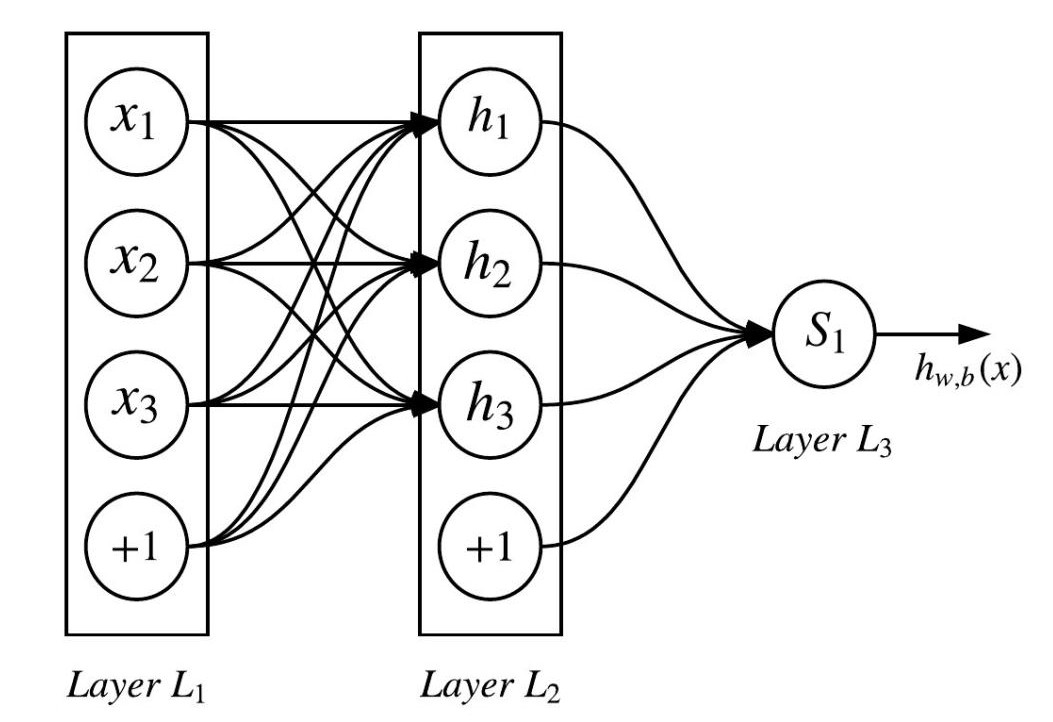
\includegraphics[width=0.80\textwidth]{FFNN}
    \caption{شبکه عصبی \lr{Feedforward}}
    \label{fig:ffnn}
\end{figure}

بر اساس توپولوژی شبکه، شبکه‌های عصبی به دو نوع 
\lr{Feedforward}
و
\lr{Recurrent/Recursive}
تقسیم می‌شوند که می‌توان با ترکیب آن‌ها به شبکه‌های ترکیب شده نیز دست یافت.
یک نمونه ساده از شبکه‌های عصبی
\lr{Feedforward}
در شکل
\ref{fig:ffnn}
آمده‌است. این شبکه دارای ۳ لایه مختلف است، لایه‌ی
\lr{L1}
لایه‌ی ورودی و دریافت کننده وکتور ورودی است. لایه‌ی
\lr{L1}
لایه‌ی میانی و به اصطلاح پنهان که خروجی لایه‌ی اول را گرفته و خروجی آن به لایه‌ی بعدی داده می‌شود. لایه نهایی نیز لایه‌ی
خروجی است که نتیجه‌ی شبکه‌ی عصبی میباشد.
دایره‌ها نشان دهنده‌ی نورون‌ها می‌باشند که به آن‌ها
\lr{Activation function}
نیز گفته می‌شود. خطوط میان هر دو نرون نشان دهنده ارتباطی برای جریان اطلاعات است. هر خط با یک بردار وزن کنترل می‌شود
که میزان اثر گذاری سیگنال بین هر دو نورون را تایین می‌کند.

\subsection{\lr{Activation functions}}

اگر به درون هر لایه برویم خواهیم دید که این لایه‌ها ورودی لایه‌ی قبلی را گرفته و خروجی را با استفاده از فرمول زیر
محاسبه می‌کند.
\begin{equation}
    f(W^tx)=f(\sum_{i=1}^{inputs} W_ix_i + b)
    \label{formula:activation}
\end{equation}

برای تابع
f
در فرمول
\ref{formula:activation}
کاندیدهای مختلفی وجود دارد که به بررسی برخی از آن‌ها می‌پردازیم.

\subsubsection{sigmoid}

این تابع یکی از معروف‌ترین توابع برای استفاده جهت
\lr{Activation function}
‌است. تابع سیگموید ورودی حقیقی را دزیافت می‌کند و عددی میان ۰ و ۱ تولید می‌کند. این تابع در انواع کاربرد‌های شبکه‌‌های
عصبی استفاده‌ی زیادی دارد و دلیل آن امکان استفاده از مفهوم درست و غلط باینری با استفاده از نتیجه می‌باشد. بدین شکل که
عدد ۱ به معنای درست و عدد ۰ به معنای غلط می‌شود.

\begin{equation}
    sigmoid(W^tx) = \dfrac{1}{1 + exp(W^tx)}
\label{formula:sigmoid}
\end{equation}

اما غیر خطی بودن
sigmoid
سبب شده‌است که این تابع به تازگی محبوبیت خود را از دست بدهد زیرا امکان گیر کردن در نقاطی که گرادیان ۰ است وجود دارد.

\begin{figure}[h]
    \centering
    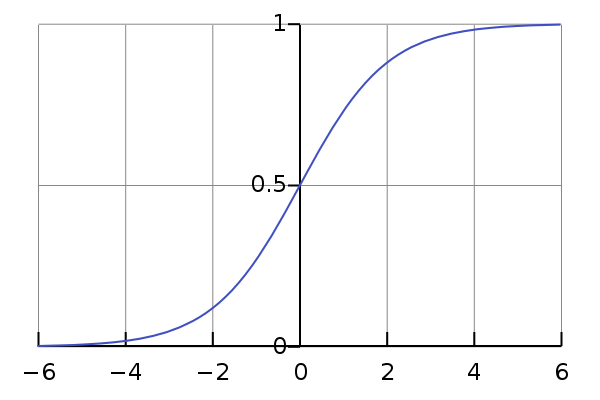
\includegraphics[width=0.80\textwidth]{sigmoid}
    \caption{تابع \lr{sigmoid}}
    \label{fig:sigmoid}
\end{figure}

مشکل دیگر این تابع این است که خروجی آن با مرکزیت ۰ نمی‌باشد. این مسئله سبب به وجود آمدن حالت زیگزاکی
تا در هنگام به روزرسانی وزن‌ها در زمان یادگیری شود.

\subsubsection{tanh}

این تابع در عمل بیشتر ترجیح داده می‌شود زیرا خروجی آن با مرکزیت عدد ۰ است و بازه‌ی خروجی
tanh
بین
\lr{-۱}
تا ۱ می‌باشد.

\begin{equation}
    tanh(W^tx) = \dfrac{e^{W^tx} -e^{-W^tx}}{e^{W^tx} + e^{-W^tx}}
\label{formula:tanh}
\end{equation}

\subsubsection{ReLU}

این تابع نیز از محبوبیت بالایی برخوردار است و دلیل آن سادگی محاسبه‌ی آن می‌باشد و سرعت آن در رسیدن به نتیجه در زمان
یادگیری میباشد. این تابع در اکثر مواقع نتایجی با عملکرد برابر یا بهتر نسبت به توابع
sigmoid
و
tanh
دارد و با توجه به سادگی آن معمولا به دو تابع دیگر ترجیح داده می‌شود.

\begin{equation}
    ReLU(W^tx) = \max(0, W^tx)
\label{formula:relu}
\end{equation}

\subsubsection{softmax}

از تابع
softmax
می‌توان به عنوان
\lr{Activation function}
لایه‌ی اخر استفاده کرد. این تابع حالت کلی تابع تابع
logistic
است که یک بردار
k
بعدی با مقادیر حقیقی را دریافت می‌کند و یک بردار
k
بعدی که هر کدام از عناصر آن عددی بین ۰ و ۱ دارند تولید می‌کند. به طور معمول از
softmax
در لایه‌ی آخر شبکه‌های
Feedforward
و همچنین عمل
classification
استفاده می‌شود.

\begin{equation}
   \sigma(X)_j = \dfrac{e^{x_j}}{\sum_{k = 1}^{K} e^{x_k} }  \mbox{ for i = 1,...,n }
\label{formula:softmax}
\end{equation}

\subsection{یادگیری}

برای انجام فرایند یادگیری در یک شبکه‌ی عصبی به طور معمول از
\lr{Stochastic gradient descent}
به همراه
\lr{Backpropagation}
برای کاهش خطای شبکه استفاده می‌شود. گرادیان
\lr{Loss function}
یا همان خطای شبکه در ابتدا برای وزن‌های میان آخرین لایه پنهان و لایه خروجی محاسبه می‌شود، به همین ترتیب گرادیان
مربوط به وزن‌های لایه‌های قبلی به صورت بازگشتی با اعمال کردن قاعده زنجیری محاسبه می‌شوند.
با استفاده از این اعداد محاسبه شده وزت‌های هر لایه به روزرسانی می‌شوند. این کار می‌تواند به صورت
iterative
ادامه یابد تا عمل یادگیری به شرایط پایان برسد.

\section{یادگیری عمیق}
در اواخر دهه 90 میلادی جامعه‌ی تحقیقاتی علاقه‌ی خود را به شبکه‌های عصبی از دست داد. دلیل آن هم استفاده از شبکه‌های
با عمق کم
(Shallow)
بود زیرا استفاده از شبکه‌های عمیق
(Deep)
بسیار پیچیده بود و هزینه‌ی محاسباتی زیادی می‌برد.

اما به طور ناگهانی با بهتر شدن سخت افزار و به روز شدن آن‌ها یادگیری عمیق سبب رسیدن به نتایج پیشرفته‌ای در زمینه‌های مختلف شد.
شروع این تغییرات در زمینه بینای ماشین شکل گرفت و سپس به شناسایی گفتار راه یافت. در سال‌های اخیر این روش در تکنیک‌های
مربوط به پردازش زبان و گفتار به شدت مورد استفاده قرار گرفت.

این انقلاب شبکه‌های عمیق می‌تواند دلایل مختلفی داشته باشد اما مهم‌ترین آن‌ها عبارتند از:

\begin{enumerate}
	\item رشد سخت افزار و افزایش قدرت محاسباتی
	\item وجود حجم زیادی از داده به منظور یادگیری
	\item قدرت و انعطاف یادگیری عمیق
\end{enumerate}

به طور خلاصه یادگیری عمیق از به هم چسباندن تعدادی لایه‌ی محاسباتی غیر خطی استفاده می‌کند تا ویژگی‌ها را استخراج و تبدیل کند.
لایه‌های نزدیک به ورودی اطلاعات ساده را استخراج می‌کنند و هر چه به لایه‌های جلو تر نزدیک می‌شویم ویژگی‌های پیچیده تر
از ویژگی‌های ساده استخراج می‌شوند.

\section{رویکردها}

\subsection{پردازش زبان طبیعی}

پردازش زبان و گفتار طبیعی زیرشاخه‌ای از علوم کامپیوتر، هوش مصنوعی و زبان‌شناسی است که هدف آن درک زبان طبیعی با
استفاده از کامپیوتر است. بسیاری از الگوریتم‌های متن کاوی به طور گسترده از تکنیک‌های
NLP
مثل
\lr{Part of Speech Tagging}
استفاده می‌کنند\cite{DBLP:journals/corr/AllahyariPASTGK17a}.

\subsection{\lr{Information Extraction}}

عمل 
\lr{information extraction}
به استخراج اتوماتیک اطلاعات یا حقایق از اسناد بدون ساختار یا نیمه ساختارمند گفته می‌شود.
این عمل معمولا به عنوان نقطه شروعی برای دیگر الگوریتم‌های متن کاوی استفاده می‌شود. به عنوان مثال استخراج
موجودیت‌ها و روابط آن‌ها از متن که می‌تواند اطلاعات معنایی مفیدی به ما بدهند یکی از کار‌های صورت گرفته
در این رویکرد است\cite{DBLP:journals/corr/AllahyariPASTGK17a}.

\subsection{خلاصه سازی متن}

خلاصه سازی متن یا
\lr{Text Summation}
روشی است که در بسیاری از کاربرد‌های متن کاوی به آن نیاز است تا بتوانند با استفاده از خلاصه‌ی یک متن بلند
یا تعدادی متن به مروری اجمالی دست یافت.

به طور کل دو روش خلاصه سازی وجود دارد،
\lr{extractive summarization}
که خلاصه‌ی به دست آمده شامل واحد‌های اطلاعاتی است که از متون اصلی استخراج شده. در مقابل
\lr{abstractive summarization}
وجود دارد که خلاصه به دست آمده ممکم است شامل اطلاعاتی باشد که در اسناد اصلی موجود نباشند\cite{DBLP:journals/corr/AllahyariPASTGK17a}.

\subsection{تحلیل احساسات و عواطف}

\lr{Sentiment analysis}
یا
\lr{Opinion Mining}
در واقع بررسی کامپیوتری نظرات، احساسات، عواطف، ارزیابی‌ها و رفتار مردم در مقابل موجودیت‌هایی
مثل محصولات، سرویس‌ها، سازمان‌ها، اشخاص، مشکلات، رویدادها و مسائل و ویژگی‌های مربوط به آن‌هاست.
رشد سریع
\lr{Sentiment analysis}
به دلیل همزمانی آن با به وجود آمدن شبکه‌های اجتماعی مانند فروم‌های نقد و بررسی، بلاگ‌های بحث و جدل،
شبکه‌های اجتماعی، فیسبوک، توییتر و غیره بود زیرا برای اولین بار در تاریخ محققان به حجم عظیمی
از داده‌های نظرات مردم دست یافتند.
\cite{zhang2018deep}

با ظهور تجارت الکترونیک و فروشگاه‌های آنلاین مقدار زیادی از متون مربوط به این حوزه تولید و روز به روز
به حجم این متون اضافه می‌شود. بررسی نظرات و تحلیل احساسات کاربران در این صنعت و با استفاده از داده‌های به دست
آمده از بررسی کالاهای مختلف توسط افراد یا نظرات آن‌ها می‌تواند منجر به پیشرفت تبلیغات و بازاریابی آنلاین شود\cite{DBLP:journals/corr/AllahyariPASTGK17a}.

متونی که برای استخراج عواطف استاده می‌شوند اغلب در سه سطح مورد بررسی قرار می‌گیرند: سطح سند، سطح جمله و سطح جنبه و نمود.
در سطح سند کل یک متن به عنوان منبع بررسی عواطف و احساسات در نظر گرفته می‌شود و مثبت یا منفی بودن آن
به طور کلی بیان می‌شود. برای رسیدن به این هدف فرض می‌شود که کل سند یک واحد اطلاعاتی ساده است و در آن
نظراتی در مورد
\textbf{یک}
مسئله وجود دارد.
\cite{zhang2018deep}

در سطح جمله هر جمله به صورت جدا بررسی می‌شود و تشخیص داده می‌شود که آیا جمله‌ی بررسی شده حاوی نظری مثبت، منفی
یا خنثی است. آنالیز در این سطح رابطه‌ی تنگاتنگی با
\lr{Subjectively Classificaion}
دارد که جمله‌های دارای اطلاعات حقیقی را از جملاتی که حاوی نظرات هستند متمایز می‌کند. اما نکته‌ای که وجود دارد آن است که
نمی‌توان گفت جملاتی که برای انتقال حقایق ساخته شده‌اند حاوی احساسات نیستند.
\cite{zhang2018deep}

تجزیه و تحلیل احساسات مبتنی بر جنبه، در اسناد به دنبال نظرات در مورد بخشی خاص می‌گردد. به عنوان مثال در یک نظر
مربوط به یک کالا، ممکن است فرد از قسمت‌هایی ناراضی و از قسمت‌هایی از کالا راضی باشد، اما به طور کلی نظر مثبتی
ثبت کرده باشد. هدف از این کار بررسی جوانب مختلف یک به اصطلاح
target
است.
\cite{zhang2018deep}

\subsection{خوشه بندی متن}

خوشه بندی
\lr{(Clustering)}
یکی از روش‌های پر استفاده در یادگیری نظارت نشده در متن کاوی است. خوشه بندی عمل تقسیم داده‌ها به گروه‌های
(خوشه)
مختلف است به طوری که داده‌های هر گروه شباهت بیشتری با یکدیگر نسبت به داده‌های گروه‌های دیگر داشته باشند\cite{DBLP:journals/corr/AllahyariPASTGK17a}.


\subsection{طبقه‌بندی متن}

طبقه بندی متن یا 
\lr{Text Classification}
یک موضوع کلاسیک در پردازش زبان‌های طبیعی است که در آن نیاز است تا اسناد مختلف را در گروه‌های
از پیش تعیین شده‌ی موجود قرار داد\cite{c9d4fbeac7324056bed5d1cb262a7268}.
این موضوع به دلیل کاربرد‌های مختلف آن مانند جست و جو در وب، بازیابی اطلاعات،
رتبه بندی و طبقه بندی اسناد از اهمیت بالای برخوردار است\cite{joulin2016fasttext}.

در سال‌های اخیر نشان داده شده است که شبکه‌های عصبی که می توانند از ترتیب کلمات استفاده کنند،
برای دسته بندی متن موثر هستند\cite{iyyer-etal-2015-deep}.

\subsection{ترجمه ماشینی عصبی}
ترجمه ماشینی عصبی یا
\lr{Neural Machine Translation}
یک روش برای رفع نواقض ترجمه ماشینی سنتی است. در این روش متن ورودی به صورت مستقیم و
\lr{end-to-end}
برای ترجمه یادگیری و به متن خروجی تبدیل می‌شود.
به طور کلی شبکه‌هایی که این مسئولیت را بر عهده دارند از دو شبکه
RNN
تشکیل شده‌اند. یکی برای پردازش متن و دیگری برای تولید متن خروجی.
بسیاری از اوقات از مکانیزم توجه برای این کار استفاده می‌شود.
این کار سبب بهبود عملکرد در برابر جملات و دنباله‌های طولامی می‌شود.

مشکلات اصلی استفاده از شبکه‌های عمیق به جای استفاده از مدل‌های آماری به سه دسته‌ی کلی طبقه بندی می‌شود.
اولین مشکل زمان زیاد مربوط به بخش یادگیری است که این مسئله برای تمام روش‌های شبکه‌های عمیق وجود دارد.
مشکل بعدی عدم ثبات در مواجهه با کلماتی است که به ندرت استفاده می‌شوند.
و آخرین مشکل آن است که این نوع شبکه‌ها در برخی موارد قادر به ترجمه‌ی تمام کلمات ورودی نیستند.\cite{wu2016google}


\section{شبکه‌ها}

\subsection{Autoencoders}

شبکه عصبی
Autoencoder
یک شبکه سه لایه است که اندازه ابعاد خروجی آن با ابعاد ورودی برابر است. شکل 
\ref{fig:autoencoder}
ساختار یک
Autoencoder
را نشان می‌دهد.

\begin{figure}[h]
    \centering
    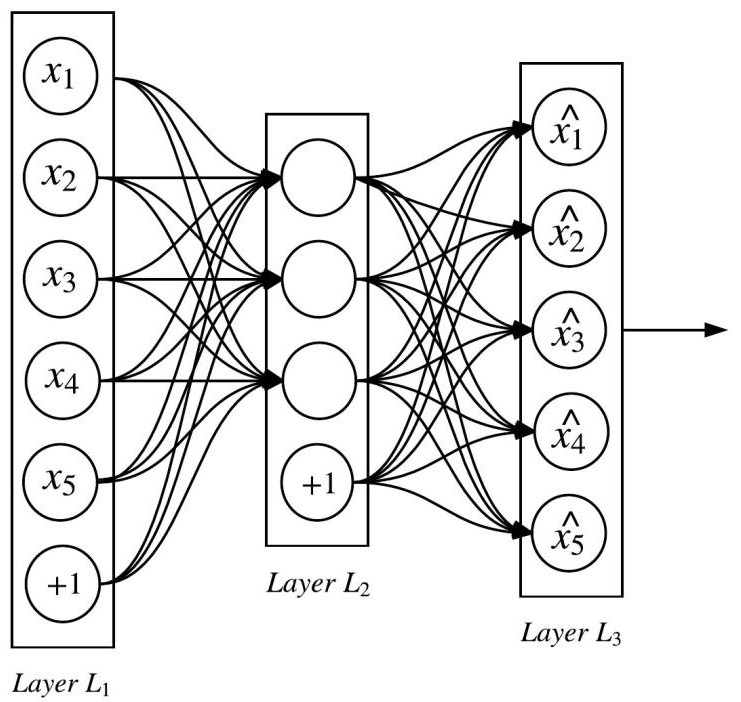
\includegraphics[width=0.80\textwidth]{autoencoder}
    \caption{شبکه عصبی autoencoder}
    \label{fig:autoencoder}
\end{figure}

در این نوع شبکه ورودی ابتدا به یک لایه‌ی پنهان به اصطلاح
encode
می‌شوند سپس خروجی این لایه 
decode
می‌شود و به لایه‌ی خروجی می‌رسد. هدف این نوع شبکه‌ها یادگیری ارائه‌ و نمایش ورودی می‌باشد. اتوانکودرها قادر به یادگیری
نمایش‌های غیر خطی می‌باشدن که نسبت به روش‌های خطی مثل
PCA
یا
LSA
از برتری برخوردار است.

\subsection{طبقه بندی کننده خطی}

طبقه بندی کننده‌ی خطی یا
\lr{Linear Classifier}
به عنوان روشی قوی و پایه‌ای برای مسائل طبقه بندی متون مورد قبول همه واقع شده‌اند. بر خلاف
سادگی ساختاری این شبکه‌ها، در صورت استفاده از ویژگی‌های درست و مناسب می‌توانند به نتایج مطلوبی
دست‌ یابند. ویژگی دیگر مهم این شبکه‌ها عملکرد مناسب در هنگام استفاده از دیتاست‌های بزرگ می‌باشد\cite{joulin2016fasttext}.

طبقه بندی کنندگان خطی پارامترها را بین کلاس‌ها و ویژگی‌ها به اشتراک نمی‌گذارند و این سبب ضعیف عمل
کردن در امر
\lr{Generalization}
هنگامی که تعداد کلاس‌ها بالا می‌رود و برخی از کلاس‌ها نمونه‌های کمی دارند می‌شود.

\subsection{شبکه \lr{Convolutional}}

\lr{CNN}
یک شبکه
\lr{feedforward}
با لایه‌های کانولوشنال در هم تنیده شده با لایه‌های
\lr{pooling}
است. در این شبکه‌ها لایه‌ی کانولوشنال هر بخش از دیتای ورودی شبکه یا خروجی لایه‌ی قبل را به یک بردار 
تبدیل می‌کند که این انر امکان پردازش موازی را نیز فراهم می‌کند\cite{iyyer-etal-2015-deep}. شکل
\ref{fig:cnn}
یک شبکه کانولوشنال ساده را نشان می‌دهد.

بسیاری از محققان بدین مسئله دست یافته‌اند که استفاده از شبکه‌های کانولوشنال
(\lr{ConvNets})
برای استخراج اطلاعات از سیگنال‌های پردازش نشده بسیار مناسب می‌باشد. به همین دلیل این شبکه‌ها
استفاده‌ی زیادی در
\lr{Computer Vision}
،
\lr{Speech Recognition}
و غیره دارند\cite{c9d4fbeac7324056bed5d1cb262a7268}.

بسیاری برای کار کردن در زمینه متن‌کاوی، به متون به شکل سیگنال‌های پردازش نشده نگاه می‌کنند
تا بتوانند با استفاده از
\lr{ConvNets}
اطلاعات ارزشمند و مختلفی از متون استخراج کنند\cite{c9d4fbeac7324056bed5d1cb262a7268}.

CNN is a neural network that can make useof the internal structure of data 
such as the2D struc-tureof image data through convolution layers, whereeach 
computation unit responds to a small region ofinput  data  (e.g.,  a  small  
square  of  a  large  image)
\cite{johnson-zhang-2015-effective}

\begin{figure}[h]
    \centering
    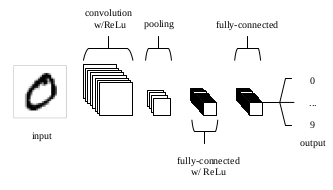
\includegraphics[width=0.80\textwidth]{CNN}
    \caption{ساختار یک شبکه عصبی کانولوشنال ساده}
    \label{fig:cnn}
\end{figure}

\subsection{\lr{RNN}}

\lr{RNN}
مخفف
\lr{Recurrent Neural Network}
می‌باشد. این شبکه‌ها دارای حلقه‌های
\lr{feedback}
در لایه‌های خود هستند. همین ویژگی اجازه می‌دهد تا داده را با گذشت زمان در حافظه‌ی خود نگه دارند.
اما یادگیری این نوع شبکه‌ها برای مسائلی که نیاز به یادگیری وابستگی‌های طولانی مدت دارند سخت است.

در یک شبکه
\lr{RNN}
به طور معمول در انجام فعالیت‌های مربوط به پردازش متن هر واحد شبکه کلمه‌ی ورودی را به همراه
خروجی تولید شده‌ی خود برای کلمه‌ی گذشته را پردازش می‌کند. این ویژگی از پردازش موازی جلوگیری می‌مند\cite{iyyer-etal-2015-deep}.

در تحقیقی که برای مقایسه
\lr{RNN}
و
\lr{CNN}
جهت رسیدن به دستورعملی ابتدایی برای انتخاب شبکه عمیق در راستای انحام فعالیت‌های مربوط به زبان طبیعی
انجام شد، نشان داده شد که شبکه‌های
\lr{RNN}
در تعداد زیادی از مسائل عملکردی مناسب و قوی دارند. همچنین در این تحقیق بر اهمیت زیاد به دست آوردن
مقادیر مناسب
\lr{batch size}
و
\lr{hidden size}
تاکید بسیار شده‌است\cite{8844895}.

\begin{figure}[h]
    \centering
    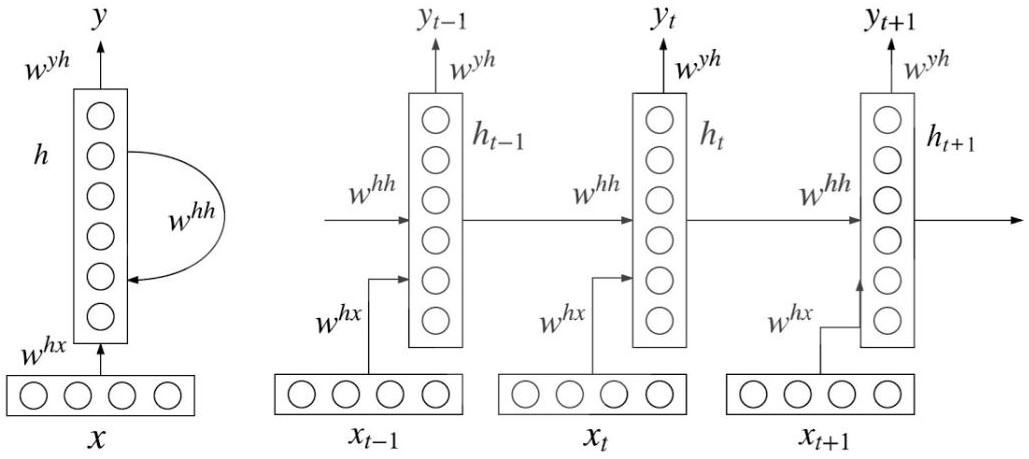
\includegraphics[width=0.8\textwidth]{rnn}
    \caption{ساختار یک شبکه عصبی Recurrent}
    \label{fig:rnn}
\end{figure}

\subsection{LSTM}

\lr{LSTM}
مخفف
\lr{Long-Short Term Memory}
است. این شبکه‌ها در واقع نوع خاصی از شبکه‌های
\lr{RNN}
هستند که علاوه بر ساختار اصلی از واحد‌های ویژه‌ای
(\lr{special units})
استفاده می‌کنند. این واحدها در خود یک سلول حافظه
(\lr{memory cell})
جای داده‌اند که می‌تواند داده را برای مدت زمان طولانی در خود ذخیره کند.

مجموعه‌ای از گیت‌ها جهت تنظیم داده‌های ورودی به حافظه، داده‌های خروجی و داده‌های فراموش شده طراحی
شده‌اند. این روش طراحی به مدل اجاره می‌دهد که وابستگی‌های طولانی مدت‌تری را یادگیری کند\cite{8844895}.

\begin{figure}[h]
    \centering
    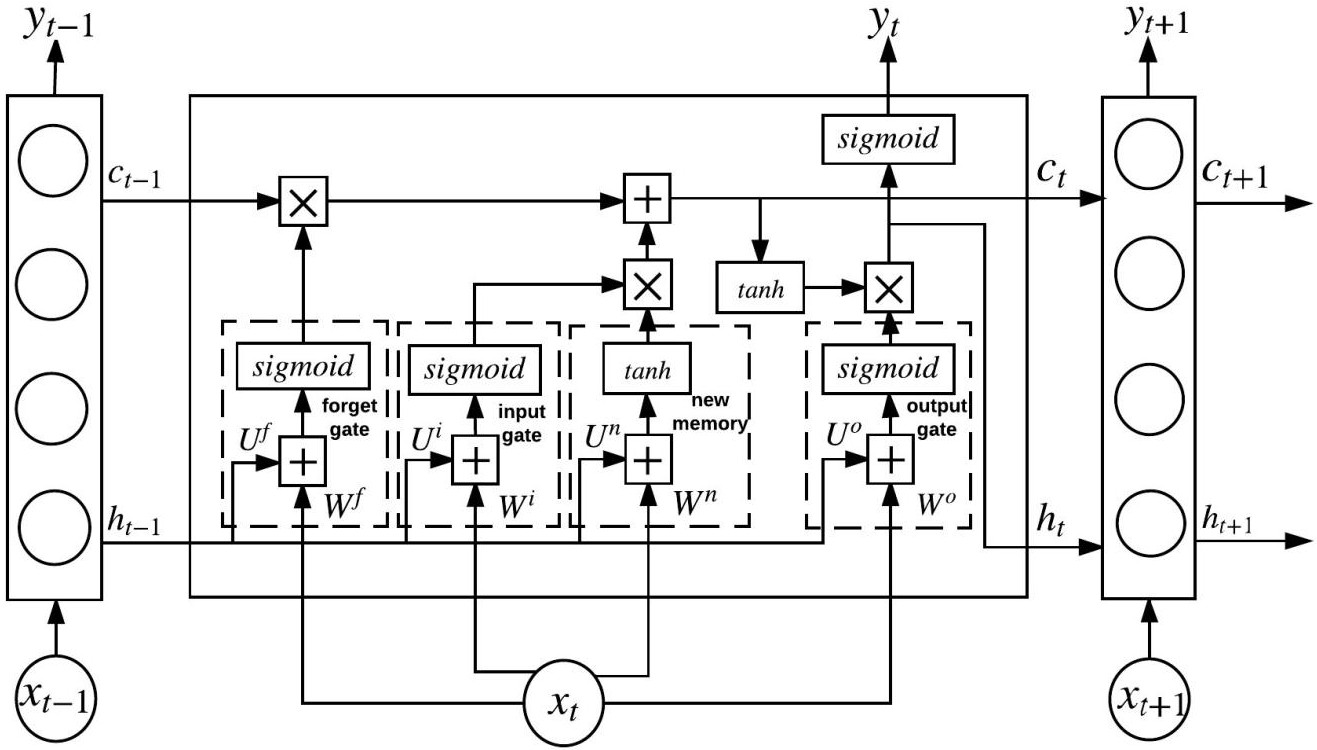
\includegraphics[width=0.8\textwidth]{lstm}
    \caption{ساختار یک شبکه عصبی LSTM}
    \label{fig:lstm}
\end{figure}

\subsection{مکانیزم توجه}

اگرچه شبکه‌های
RNN
و
LSTM
می توانند واستگی‌های زمانی را درک کنند اما در عمل کار کردن با این نوع وابستگی‌ها بسیار مشکل می‌باید. برای گذر از این
مشکل تکنیکی به نام
\lr{attention mechanism}
معرفی شد. این تکنیک با الهام گیری از مکانیزم توجه در سیستم بینایی انسان‌ها ساخته شده‌است. توجه بینایی انسان قادر است
تا بر بخشی از تصویر تمرکز کند و آن را با وضوح و رزلوشن بالا ببیند در حالی که اطراف این ناحیه با رزلوشن پایین تری دیده می‌شود.
این ناحیه تمرکز با گذر زمان تنظیم می‌شود.

در پردازش زبان و گفتار مکانیزم توجه به مدل این اجازه را می‌دهد تا توجه خود را به آن چه تا کنون توسط متن ورودی تولید شده‌است
متمرکز کند. بر خلاف
RNN
و
LSTM
که متن را به یک بردار با طول ثابت تبدیل می‌کنند.

\subsection{شبکه‌های \lr{Transformer}}
به تازگی شبکه‌های
Transformer
نتایج و موفقیت‌های زیادی در بسیاری از کاربرد‌های هوش مصنوعی مثل پردازش زبان و گفتار، بینایی ماشین و
پردازش صدا و امواج کسب کرده‌اند. همین مسئله سبب آن شده‌است که محققین زیادی کار بر روی این شبکه‌ها را آغاز کنند
در نتیجه پیشرفت‌های چشم‌گیری حاصل شده‌است.

Transformer
ها یکی از روش‌های
\lr{deep learning}
هستند که استفاده‌های مختلفی از آن‌ها می‌شود. این شبکه‌ها در اصل به عنوان مدلی برای داده‌های دنباله‌ای به خصوص
ترجمه ماشینی ارائه شدند. پژوهش‌های بعدی نشان داد که مدل‌های از پیش
train
شده‌ی مبتنی بر
transformer
ها قادر به کسب نتایج فوق‌العاده در بسیاری از مسائل هستند. همین مسئله باعث شد تا شبکه‌های
transformer
به عنوان معماری پایه‌ی بسیاری از مسائل پردازش زبان و گفتار طبیعی استفاده شوند.

مدل ابتدایی که یک مدل
sequence-to-sequence
است شامل یک
encoder
و یک
decoder
می‌باشد که هر کدام از این بخش‌ها تشکیل شده از تعدادی بلاک دقیقا شبیه به هم هستند. هر
encoder
به طور کلی تشکیل شده از یک ماژول
multi-head
و یک ماژول
self-attention
و یک شبکه 
feed-forward
است. در مقابل در بلاک
decoder
یک ماژول
cross-attention
بین هر دو جفت ماژول از ماژول‌های گفته شده قرار دارد.\cite{lin2021survey}

\begin{figure}[h]
    \centering
    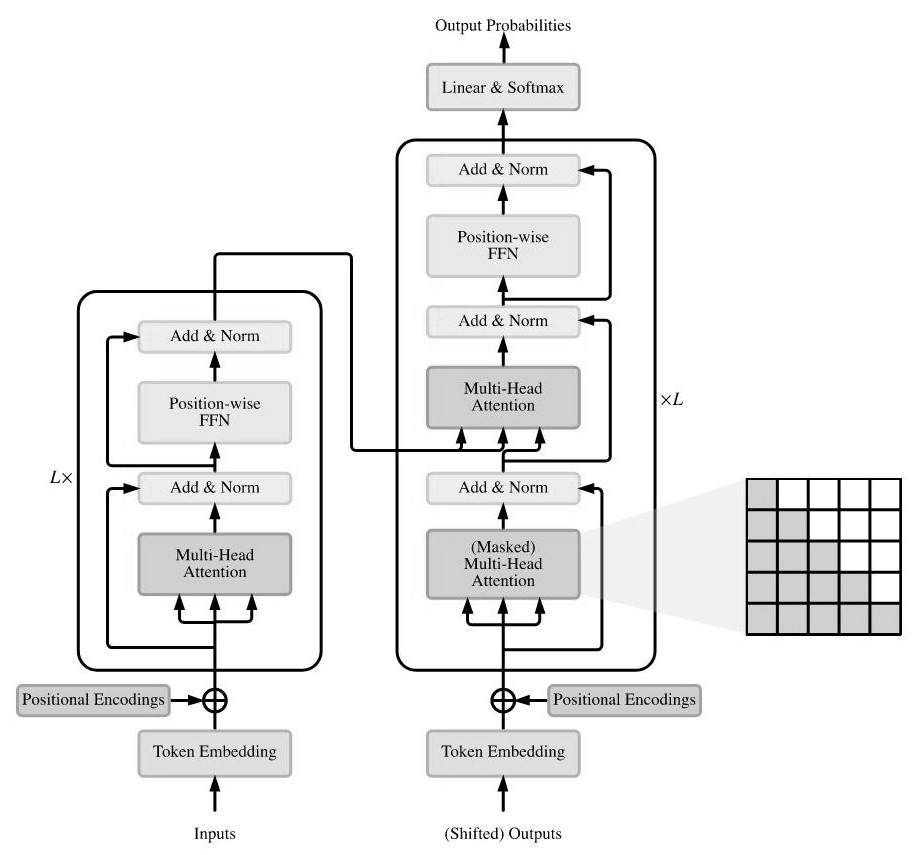
\includegraphics[width=0.8\textwidth]{transformer}
    \caption{ ساختار شبکه transformer }
    \label{fig:transformer}
\end{figure}

\subsubsection{شبکه‌ی BERT}

شبکه‌ی
BERT
که مخفف
\lr{Bidirectional Encoder Representations from Transformers}
است در بسیاری از موارد و مسائل مربوط به پردازش زبان و گفتار طبیعی استفاده می‌شود.
این شبکه طوری طراحی شده‌است تا با داده‌های برچسب گذاری نشده کار کند. همین مسئله بائث می‌شود تا بتوان با استفاده از
fine-tuning
مدل
BERT
را در بسیاری از موارد به خصوص جواب دادن به سوالات مورد استفاده قرار داد. 

این مدل از دو مرحله‌ی
pre-training
و
fine-tuning
تشکیل شده‌است. در مرحله‌ی اول مدل با استفاده از داده‌های برچسب گذاری نشده یادگیری می‌شود و در مرحله بعدی پارامتر‌های
یادگیری شده به مدل داده می‌شود و با استفاده از داده‌های برچسب گذاری شده و یک لایه‌ی نهایی
fine-tune
می‌شود. اگرچه پارامتر‌های یادگیری شده ثابت هستند اما این شبکه برای دست‌یابی به مدل مناسب باید برای هر مسئله
fine-tune
شود. مزیت
BERT
نیز همین است که ساختار شبکه‌های مختلف با توجه به لایه‌ی آخری که اضافه می‌شود شباهت‌های بسیاری دارند و تنها نیاز است
تا تغییرات کوچکی ایجاد شود.

ساختار شبکه‌ی
transformer
به کار رفته به مدل اصلی بسیار شبیه است. اما معماری کلی شبکه به صورت یک شبکه‌ی چندلایه‌ی
\lr{transformer encoder}
است. 

برای آن که این شبکه قادر به انجام وظایف زیادی باشد ورودی شبکه طوری طراحی شده‌است تا امکان دریافت جمله و جفت جمله
را داشته باشد. البته در اینجا جمله به معنای متن ورودی است.
در این شبکه برای توکن کردن داده از روش
WordPiece
با تعداد ۳۰۰۰۰ لغت استفاده شده‌است. اولین توکن هر دنباله نیز
CLS
در نظر گرفته شده تا با استفاده از آخرین
\lr{hidden state}
مربوط به این توکن بتوان وظایف مربوط به طبقه بندی را انجام داد.
همچنین در صورتی که داده به صورت جفت جمله باشد، هر دوی این جملات با هم ترکیب شده و به صورت یک دنباله در می‌ایند.
برای آن که این دو جمله در دنباله تولید شده از هم متمایز باشند از توکن
SEP
میان آن‌ها استفاده می‌شود. در انتها در توکن ورودی به ترکیبی از توکن،
segment
مربوط به آن(جمله‌ی اول یا دوم)
و همچنین مکان توکن در جمله تبدیل می‌شود.

به منظور
pre-train
کردن شبکه‌ به جای استفاده از روش‌های سنتی چپ به راست یا راست به چپ از دو مسئله بدون نظارت بهره گیری می‌شود.

مسئله‌ی اول
\lr{Masked Language Modeling}
است. برای این کار بخشی از توکن‌های ورودی به اصطلاح
mask
می‌شوند. این کار به صورت رندم و با درصدی از پیش تعیین شده صورت می‌گیرد. سپس شبکه به پیشبینی توکن‌های پنهان شده
که با 
MASK
نشان داده می‌شوند می‌پردازد. بردار نهایی به دست آمده از این کار به یک تابع
softmax
داده می‌شود. در این مدل ۱۵ درصد توکن‌ها به صورت رندم پنهان‌سازی می‌شوند و همچنین به جای پیشبینی کل دنباله تنها
توکن‌های پنهان شده پیشبینی می‌شوند. هنگام پنهان کردن توکن‌ها ۳ اتفاق ممکان است رخ دهد. با احتمال ۸۰ درصد توکن
پنهان می‌شود. با احتمال ۱۰ درصد توکن پیگری که به صورت رندم انتخاب شده‌است جایگذاری می‌شود. و با احتمال ۱۰ درصد
بدون تغییر باقی می‌ماند. سپس مرحله پیشبینی با بهره گیری از
\lr{cross entropy loss}
انجام می‌شود.

مسئله‌ی دوم پیشبینی جمله‌ی بعدی است. بسیاری از مسائل پردازش زبان و گفتار مانند پاسخ دهی به سوالات نیازمند داشتن
دانشی از ارتباط بین دو جمله است. برای آن که شبکه درکی از ارتباط میان دو جمله داشته باشد شکه با داده‌های دو جمله‌ای
یادگیری می‌شود. برای این کار دو جمله با توجه به ساختار گفته شده به شبکه داده می‌شود. در نصف مواقع جمله‌ی دوم
واقعا جمله‌ای است که در پی جمله‌ی اول می‌آید ولی در باقی موارد جمله‌ی دوم به صورت تصادفی از میان داده‌های موجود
انتخاب می‌شود.

برای انجام این دو وظیفه از دیتاست‌های
BooksCorpus
و
Wikipedia
استفاده شده‌است. 

\begin{figure}[h]
    \centering
    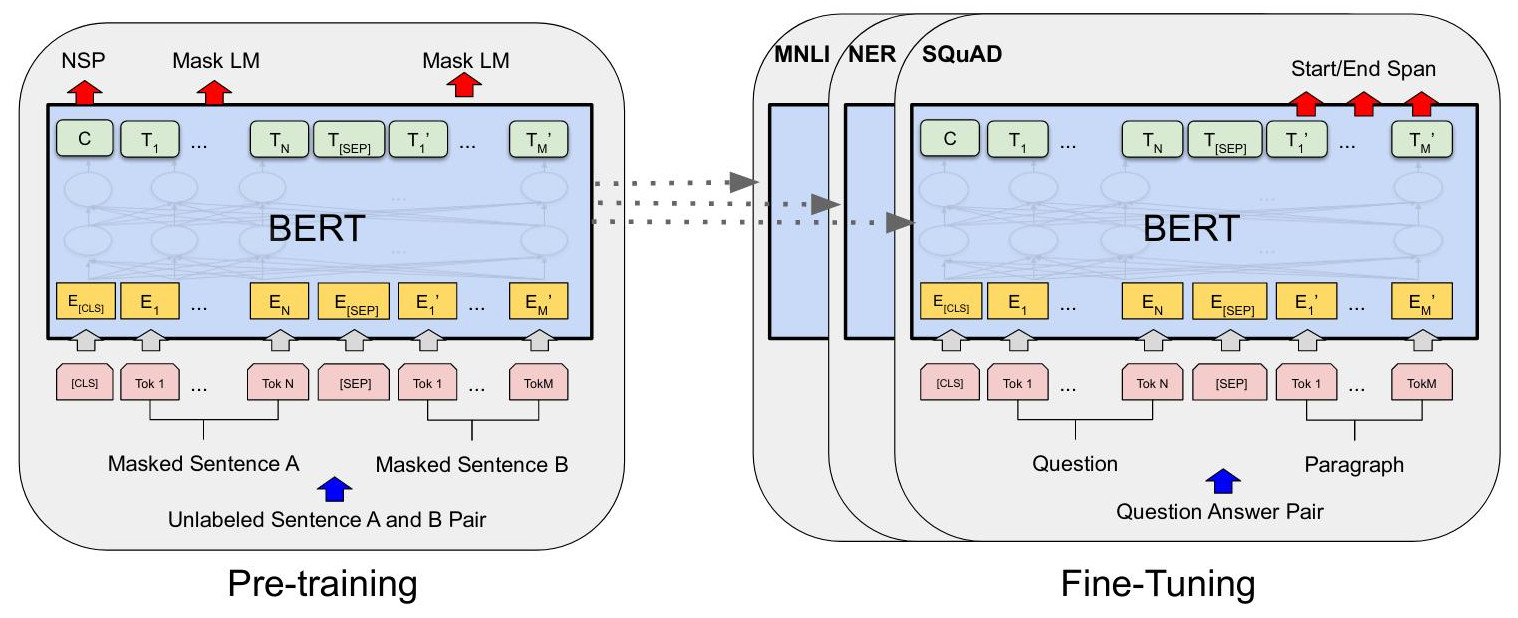
\includegraphics[width=0.8\textwidth]{bert}
    \caption{ ساختار شبکه bert }
    \label{fig:bert}
\end{figure}

بخش بعدی
fine-tune
کردن شبکه است که این کار به خاطر وجود مکانیزم توجه در شبکه به راحتی انجام می‌شود.
در واقع ورودی و خروجی‌های مورد نظر به شبکه داده می‌شود و شبکه به صورت
end-to-end
عملیات
fine-tuning
را انجام می‌دهد.

در مقایسه با
pre-training
علمیات
fine-tuning
هزینه‌ی کمتری می‌برد. به طوری که برای رسیدن به جواب با استفاده از یک
GPU
تنها چند ساعت نیاز است.\cite{devlin2018bert}



\subsection{شبکه‌های حافظه‌ای}
شبکه‌های حافظه‌ای یا
\lr{Memmory Networks}
که به طور خلاصه
MenNN
نیز نوشته می‌شوند در ابتدا برای پاسخ دهی به سوالات ارائه شدند. این شبکه دارای تعدادی کامپوننت استنباطی در کنار یک
حافظه‌ی بلند مدت بزرگ است که به عنوان منبع دانایی عمل می‌کند. وظایف کلی کامپوننت‌ها به این شکل است. کامپوننت
I
ورودی را به نمایش ویژگی‌ها تبدیل می‌کند. کامپوننت بعدی یعنی
G
بر اساس ورودی‌های دریافتی جدید حافظه را به روزرسانی می‌کند. کامپوننت
O
در واقع وظیفه‌ی تولید خروجی را بر عهده دارد و کامپوننت
R
خروجی تولید شده را به فرمت مورد نظر تبدیل می‌کند. جدول
\ref{tab:MemNN-vs-others}
مقایسه‌ی این مدل به دو شبکه
RNN
و
LSTM
را در دو مسئله با سختی‌های متفاوت نشان می‌دهد.
\cite{zhang2018deep}

\begin{table}[h]
    \begin{small}
    \begin{center}
      \begin{latin}
      \begin{tabular}{|l||l|l|l||l|l|}
        \hline
         & \multicolumn{3}{c|}{Difficulty 1} & \multicolumn{2}{c|}{Difficulty 5} \\
        \hline
        Method & actor w/o before & actor & actor+obj & actor & actor+obj \\
        \hline
        RNN & 100\% & 60.9\% & 27.9\% & 23.8\% & 17.8\% \\
        LSTM & 100\% & 64.8\% & 49.1\% & 35.2\% & 29.0\% \\
        \hline
        MemNN k= 1 & 97.8\% & 31.0\% & 24.0\% & 21.9\% & 18.5\% \\
        MemNN k= 1 & 99.9\% & 60.2\% & 42.5\% & 60.8\% & 44.4\% \\
        MemNN k= 2 & 100\% & 100\% & 100\% & 100\% & 99.9\% \\
        \hline
      \end{tabular}
      \end{latin}
      \caption{مقایسه عملکرد سه مدل حافظه‌ای}
      \label{tab:MemNN-vs-others}
    \end{center}
\end{small}
  \end{table}


\chapter{کارهای مرتبط}
\pagebreak

% طول متن برای درختواره

\begin{latin}
\begin{tiny}
\begin{noindent}
\begin{forest}
for tree = { draw },
before typesetting nodes={
    where content={}{coordinate}{},
},
forked edges,
[Text Mining,
    [Classification,
        [Sentiment Analysis
            [Autoencoder
                [\cite{zhaiEncoder}]
            ]
            [CNN\footnote{Convolutional Neural Network}
                [\cite{tang-etal-2015-document}]
                [\cite{dos2014deep}]
                [\cite{wang-etal-2016-combination}]
                [\cite{guggilla-etal-2016-cnn}]
            ]
            [GRU\footnote{Gated Recurrent Unit}
                [\cite{tang-etal-2015-document}]
                [\cite{72Zhang_Zhang_Vo_2016}]
            ]
            [LSTM\footnote{Long Short Term Memory}
                [\cite{tang-etal-2015-document}]
                [\cite{xu2016cached}]
                [\cite{yin-etal-2017-document}]
                [\cite{zhou-etal-2016-attention}]
                [\cite{wang-etal-2016-combination}]
                [\cite{guggilla-etal-2016-cnn}]
                [\cite{teng-etal-2016-context}]
                [\cite{70tang-etal-2016-effective}]
                [\cite{71ruder-etal-2016-hierarchical}]
            ]
            [MemNN\footnote{Memory Network}
                [\cite{ijcai2017-311}]
            ]
            [RecNN
                [\cite{68dong-etal-2014-adaptive}]
            ]
            [,[,[,[Sentence Level, calign=last
                    [Autoencoder
                        [\cite{socher-etal-2011-semi}]
                    ]
                    [RecNN\footnote{Recursive Neural Network}
                        [\cite{socher-etal-2011-semi}]
                        [\cite{socher-etal-2012-semantic}]
                        [\cite{socher-etal-2013-recursive}]
                        [\cite{qian-etal-2015-learning}]
                    ]
                    [CNN
                        [\cite{kalchbrenner-etal-2014-convolutional}]
                        [\cite{kim-2014-convolutional}]
                        [\cite{wang-etal-2016-dimensional}]
                        [\cite{wang-etal-2016-dimensional}]
                        [\cite{mishra-etal-2017-learning}]
                    ]
                    [LSTM
                        [\cite{wang-etal-2016-dimensional}]
                    ]
                    [RNN\footnote{Recurrent Neural Network}
                        [\cite{wang-etal-2016-dimensional}]
                    ]
            ]]]]
            [,[,[,[,[,[,[Aspect Level, calign=last         
                            [LSTM
                                [\cite{73wang-etal-2016-attention}]
                                [\cite{74YANGATT}]
                                [\cite{75liu-zhang-2017-attention}]
                            ]
                            [RNN
                                [\cite{80chen-etal-2017-recurrent}]
                            ]
                            [GRU
                            ]
                            [MemNN
                                [\cite{76tang2016aspect}]
                                [\cite{80chen-etal-2017-recurrent}]
                            ]
            ]]]]]]]
        ],
        [CNN\footnote{Convolutional Neural Network}
            [\cite{johnson-zhang-2015-effective}]
        ],
        [GRU\footnote{Gated Recurrent Unit}
            [\cite{yang-etal-2016-hierarchical}]
        ]
        [LSTM
            [\cite{graves2005framewise}]
        ]
        [Transformers
            [\cite{schmidt2020data}]
        ]
        [\cite{c9d4fbeac7324056bed5d1cb262a7268}]
        [\cite{joulin2016fasttext}]
        [\cite{iyyer-etal-2015-deep}]
        [\cite{johnson-zhang-2017-deep}]
        [\cite{DBLP:journals/corr/ConneauSBL16}]
    ],
    [Machine Translation,
        [LSTM,
            [\cite{wu2016google}]
        ]
    ]
]
\end{forest}
\end{noindent}
\end{tiny}
\end{latin}

\pagebreak

\section{مقدمه}

\section{روش‌های بر پایه رویکرد طبقه بندی متن}

\subsubsection{Seq-CNN و ‌BOW-CNN}

ترتیب کلمات درون متون قطعا تاثیر بسیار زیادی در معنا و مفهوم و در نهایت این که هر متن در چه کلاسی قرار می‌گیرد
تاثیر بسیار زیادی دارد. اما روش‌های بر مبنای
BOW
از این ویژگی استفاده‌ای نمی‌کنند. زیرا بردار حاوی اطلاعات تنها این که چه کلماتی در متن استفاده شده‌اند را نمایش می‌دهند
و ترتیب و جایگاه کلمات نادیده گرفته می‌شوند. در این مقاله برای آن که از این ترتیب بهره‌گیری و استفاده شود از شبکه‌ی عصبی
convolutional
استفاده شده‌است. استفاده از
CNN
سبب می‌شود تا بتوان از ساختار ترتیبی متون بهره برد تا هر بخش از شبکه‌ی کانولوشنی مسئولیت پردازش بخشی از متن
یا دنباله‌ای از کلمات را داشته باشد. شکل
\ref{fig:cnn-in-text}
این عمل را نشان می‌دهد.

\begin{figure}[h]
    \centering
    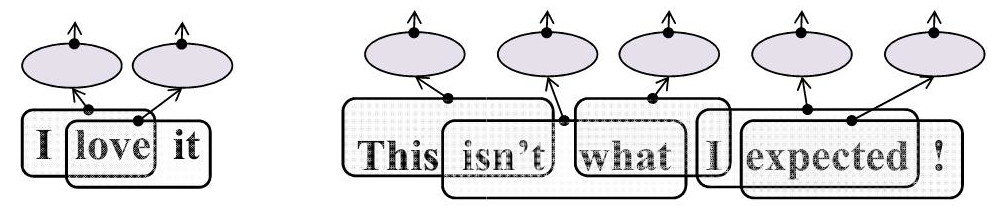
\includegraphics[width=0.8\textwidth]{cnn-in-text}
    \caption{ استفاده از شبکه‌ی کانولوشنی به منظور بهره‌گیری از ترتیب کلمات }
    \label{fig:cnn-in-text}
\end{figure}

به منظور این کار شبکه‌ی کانولوشنال به صورت مستقیم با بردار ورودی سر و کار دارد و در واقع به جای استفاده از
روش‌های
embeding
، خود شبکه این کار ار یاد می‌گیرد. دو نوع شبکه
seq-CNN
و
BOW-CNN
معرفی شد و نشان داده شد که شبکه‌ی اول در تحلیل عواطف بهتر عمل می‌کند و روش دوم در طبقه بندی بر اساس موضوع.
\cite{johnson-zhang-2015-effective}

\subsection{بررسی چند مقاله}

برای انجام عمل دسته بندی در متون در سطوح مختلف جمله، کلمه و حروف تلاش‌های زیادی انجام شد.
\cite{graves2005framewise}
در سال ۲۰۰۵ نشان داد که استفاده از شبکه‌های
lr{Bidirectional LSTM}
می‌تواند نتایجی بهتر از مدل‌های
RNN
معمولی به دست آورد. برای این کار در لایه‌های پنهان مدل ارتباطات دو طرفه اضافه کردند و با بررسی نتایج مهر تعییدی
بر عملکرد بهتر شبکه‌ی بر پایه‌ی حافظه‌ی دوطرفه زدند.

مقاله‌ی
\cite{guggilla-etal-2016-cnn}
نیز به مانند 
\cite{wang-etal-2016-combination}
از ترکیب دو شبکه‌ی
CNN
و
LSTM
برای ساخت مدل خود استفاده کرد. این مدل با بهره گیری از روش نمایش
Word2Vec
به این عمل پرداخت. هر دو شبکه‌ی کانولوشنان و دارای حافظه استفاده‌های زیادی در مسائل طبقه بندی داشته‌اند و ترکیب آن‌ها
نیز نتایج خوبی را ارائه داده است.

روش‌های محتلفی بر پایه‌ی
Transformer
ها ارائه شده‌اند. از میان این روش‌ها روش
BERT
به دلیل کاربرد بسیار و همچنین ارائه به عنوان اولین مدل موفق از نوع خود از اهمیت بالایی برخوردار است که به بررسی آن
پرداخته شد. شبکه‌های بسیاری برای بالا بردن دقت از
BERT
استفاده کرده‌اند. به طور کل در میان مقالاتی که از
Transformer
ها برای حل مسائل پردازش زبان طبیعی استفاده کرده‌اند، شبکه‌ی
BERT
جایگاه ویژه‌ای دارد.
\cite{schmidt2020data}
از سه مدل
BERT
استفاده شده‌است،
BERT-base
، مدل چندزبانه
BERT
و در آخر
SCIBERT
.
در این مدل لایه‌ی مربوط به
classification
در مدل اصلی با لایه‌ای متفا.ت جایگذاری شده‌است. این لایه همچنان خطی و
fully-connected
است، اما به جای خطای
\lr{sigmoid cross-entropy}
از
\lr{logits function}
استفاده شده‌است. این کار سبب شده‌است که مدل قادر به تخمین زدن به صورت چند کلاسه نیز باشد.

\cite{yang-etal-2016-hierarchical} 3269 2017


\section{روش‌های بر پایه رویکرد تحلیل عواطف و احساسات}

تحقیقات انجام شده روش‌های گوناگون و زیادی را برای انجام این فعالیت ارائه داده‌اند که شامل هر دو روش
نظارت شده و نظارت نشده می‌شوند.
در این تحقیقات انواع و اقسام روش‌های نظارت شده به منظور استخراج اطلاعات از نظرات کاربران
استفاده شده‌اند که می‌توان از میان آن‌ها به
\lr{Support	Vector	Machines (SVM)}
،
\lr{Maximum Entropy}
و
\lr{Naïve Bayes}
اشاره کرد.
روش‌های نظارت نشده نیز دستاورد‌های زیادی داشته‌اند.

از حدود یک دهه گذشته روش‌های مبتنی بر یادگیری عمیق پر قدرت وارد این عرصه شدند و نتایج پیشرفته‌ای
از خود در زمینه پردازش زبان و گفتار طبیعی به خصوص
\lr{Sentiment analysis}
به جای گذاشتند.
همین مسئله سبب افزایش استفاده از یادگیری عمیق در مسائل مربوط به استخراج اطلاعات و تجزیه تحلیل
عواطف و احساسات شد.
\cite{zhang2018deep}


\subsubsection{وابستگی به هدف}
در بحث استخراج و تحلیل عواطف و احساسات از متون موردی که تاثیر بسیاری در نتیجه‌ی نهایی دارد هدف یا به اصطلاح
target
می‌باشد. به عنوان مثال جمله‌ی زیر با توجه به این که هدف بررسی، سیستم عامل ویندوز باشد یا لینوکس نتیجه‌ی متفاوتی دارد.
\begin{quotation}
    لینوکس عملکرد بهتری نسبت به ویندوز دارد.
\end{quotation}
اگر هدف ما کلمه‌ی لینوکس باشد نتیجه‌ی استخراج و تحلیل متن مثبت می‌شود، و اگر هدف ویندوز باشد، نتیجه منفی است.
در صورت آن که هدف کلمه‌ی دیگری مثل اندروید باشد، نتیجه‌ی خنثی حاصل می‌شود.

مقاله‌ی
\cite{68dong-etal-2014-adaptive}
با ارائه
AdaRNN
متون را با وابستگی به هدف مورد بررسی قرار داد. این مدل با یادگیری آن که کلمه یا کلمات حاوی اطلاعات مهم را با
ربط دادن به کلمه‌ی هدف استخراج کند، متون را از دید ساختاری بررسی می‌کند.

شبکه
LSTM
می‌تواند ارتباطات معنایی بین کلمه‌ یا کلمات هدف و جملات را به دست آورد. در
\cite{70tang-etal-2016-effective}
با استفاده از این ویژگی
LSTM
دو شبکه
TD-LSTM\footnote{\lr{Target-Dependent LSTM}}
و
TC-LSTM\footnote{\lr{Target-connection LSTM}}
ارائه شد. برای این کار کلمه‌ی هدف را به عنوان یک ویژگی به شبکه‌های ایجاد شده اضافه کردند.
شبکه‌های
LSTM
قادر به درک ارتباطات معنایی درون ساختاری هستند و در فهم و پردازش ارتباطات بین جملات به خوبی عمل نمی‌کنند.
به عنوان مثال این شبکه‌ها می‌توانند پیش‌زمینه جمله را درک کنند، در جملات کیفیت غذای این رستوران بسیار بالاست.
من عاشق این رستوران هستم. کیفیت غذا پیش‌زمینه‌ی جمله‌ی مثبت بعدی است. اما پیچیدگی کنار هم
قرار گرفتن جملات مفهومی نیست که به راحتی درک شود.

در
\cite{71ruder-etal-2016-hierarchical}
مقاله با استفاده از یک شبکه حافظه بلند کوتاه مدت سلسله مراتبی دو طرفه\footnote{\lr{Hierarchical bidirectional long short-term memory}}
به شناخت و درک هر دو نوع ارتباط گفته شده پرداخته شده‌است. به دلیل وجود وابستگی مدل تنها به جمله و
ساختار آن، این شبکه را قادر به انجام پیشبینی در زبان‌های مختلف می‌سازد.

این مدل از ۳ بخش مختلف تشکیل شده‌است. بخش اول تبدیل به نمایش برداری است. هر نظری کاربران در سطح شبکه‌های
اجتماعی یا دیگر سکوهای\footnote{Platforms}
موجود ارسال می‌کنند از چند جمله تشکیل شده‌است. این جملات با استفاده از لایه گذاری\footnote{Padding}
به طول یکسان تبدیل می‌شوند. سپس هر جمله تبدیل به نمایشی از مجموعه بردارهای کلمات تشکیل دهنده آن می‌شود.
سپس هر کدام از جملات با کلمه‌ی مورد نظر و ویژگی آن (به عنوان مثال غذا\#کیفیت)
ترکیب می‌شود. به این شکل که از این دو کلمه میانگین گرفته می‌شود و به بردار اضافه می‌شود.

بخش بعدی شبکه‌ی
LSTM
است که امکان یادگیری وابستگی‌های جملات را دارد. دو شبکه‌ در ساختار وجود دارند که یکی از آن‌ها
رو به جلو است و دیگری رو به عقب.

بخش بعدی شامل دو شبکه‌ی
LSTM
دیگر است که به مانند قسمت قبل یکی رو به جلو است و دیگری رو به عقب. این دو شبکه از خروجی بخش قبلی
استفاده می‌کنند و جملات را به طور کلی و در سطح متن بررسی می‌کنند.

\begin{table}[h]
    \begin{small}
    \begin{center}
      \begin{latin}
      \begin{tabular}{|l|l|l|l|l|l|}
        \hline
        Language & Domain & Best & LSTM & H-LSTM &  HP-LSTM \\
        \hline
        English & Restaurants & 88.1 & 81.4 & 83.0 & 85.3 \\
        \hline
        Spanish & Restaurants & 83.6 & 75.7 & 79.5 & 81.8 \\
        \hline
        French & Restaurants & 78.8 & 69.8 & 73.6 & 75.4 \\
        \hline
        Russian & Restaurants & 77.9 & 73.9 & 78.1 & 77.4 \\
        \hline
        Dutch & Restaurants & 77.8 & 73.6 & 82.2 & 84.8 \\
        \hline
        Turkish & Restaurants & 84.3 & 73.6 & 76.7 & 79.2 \\
        \hline
        Arabic & Hotels & 82.7 & 80.5 & 82.8 & 82.9 \\
        \hline
        English & Laptops & 82.8 & 76.0 & 77.4 & 80.1 \\
        \hline
        Dutch & Phones & 83.3 & 81.8 & 81.3 & 83.6 \\
        \hline
        Chinese & Cameras & 80.5 & 77.6 & 78.6 & 78.8 \\
        \hline
        Chinese & Phones & 73.3 & 70.3 & 74.1 & 73.3 \\
        \hline
      \end{tabular}
      \end{latin}
      \caption{مقایسه عملکرد مدل معرفی شده با شبکه‌های دیگر}
      \label{tab:H-LSTM}
    \end{center}
\end{small}
  \end{table}

در همین راستا در
\cite{72Zhang_Zhang_Vo_2016}
شبکه‌ای در سطح جمله ارائه شد که هدف آن رفع مشکل و ضعف استفاده از
pooling
است. برای این کار از دو
GRU\footnote{\lr{Gated Recurrent Uunit}}
استفاده شده‌است. در ابتدا یک
GRU
دو طرفه\footnote{\lr{Bidirectional Gated Recurrent Uunit}}
ایجاد شده که هدف آن پردازش کلمات متن است تا
pooling
به جای آن که مستقیم بر کلمات تاثیر بگذارد به خروجی این لایه اعمال شود. سپس از یک
GRU
سه طرفه استفاده شده تا ارتباطات میان کلمه‌ی هدف و کلمات اطراف آن را درک کند.
این شبکه سه طرفه برا آن اضافه شده‌است تا بتواند ارتباطات معنایی و ساختاری متون را مدل سازی کند.
این مقاله نشان داد که استفاده از
GRU
سبب کم شدن جانب‌داری\footnote{bias}
در تصمیم گیری‌های مدل می‌شود.

\paragraph{ATAE-LSTM} \hfill \break

همانطور که گفته شد شبکه‌های
RNN\footnote{\lr{Recurrent Neural Networks}}


\subsubsection{CharSCNN و طول متن}

طول متون نیز اهمیت بالایی در نتیجه گیری بر اساس متن‌ها و دریافت عواطف و احساسات دارد.
در متون کوتاه مثل توییت‌ها یا تک جمله‌ها، به دلیل عدم وجود اطلاعات زیاد به دست آوردن تخمین درستی از
عواطف و احساسات قرار گرفته در مفاهیم متن کاری بسیار دشوار است.
برای این کار لازم است تا علوه بر داشتن دانش قبلی از استراتژی‌ها به خصوصی استفاده نمود.
در
\cite{dos2014deep}
با به کار گیری از یک شبکه‌ی عمیق کانولوشنی با نام
CharSCNN
این مشکل را حل کردند. برای این کار ابتدا کلمات متن را به صورت برداری تبدیل می‌کنند در واقع عملیات
embedding
انجام می‌شود. سپس هر بردار به دو بردار تبدیل می‌شود. یکی بردار در سطح کلمات و دیگری بردار در سطح حروف.

\begin{figure}[h]
    \centering
    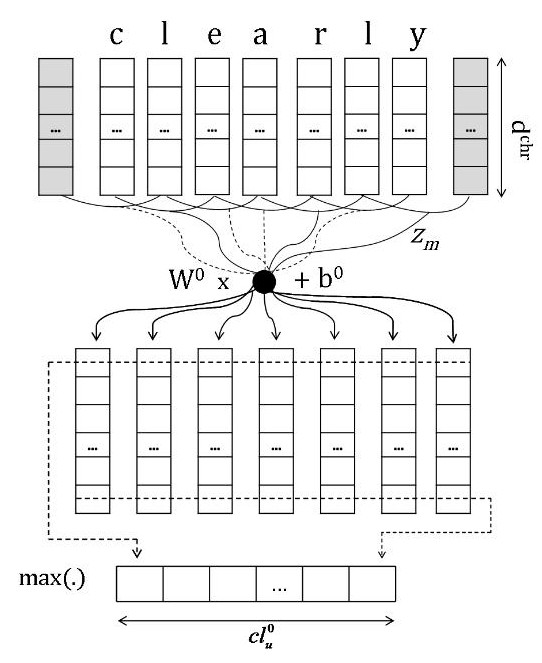
\includegraphics[width=0.5\textwidth]{CHARCNN}
    \caption{ شبکه‌ی کانولوشنی در سطح حروف }
    \label{fig:CHARCNN}
\end{figure}

در مرحله‌ی بعدی نمایش جمله‌ای از متن با استفاده از یک شبکه‌های کانولوشنی دیگر به دست می‌آید.
چالش اصلی این بخش آن است که طول جملات ثابت نیستند و قسمت‌های مهم جمله و نمایانگر عواطف و احساسات
ممکن است در هر نقطه از جمله وجود داشته باشند. این لایه، در واقع شبکه‌ی کانولوشنی است که وظیفه‌ی آن
به دست آوردن این نمایش از متن است. این کار با به دست آوردن ویژگی‌های محلی اطراف هر کلمه و ترکیب
آن‌ها با استفاده ماکزیمم گیری انجام می‌شود.



\cite{tang-etal-2015-document} 1327 2015
\cite{socher-etal-2011-semi} 1471 2011
\cite{socher-etal-2012-semantic} 1400 2012
\cite{socher-etal-2013-recursive} 5000 2013




\subsection{بررسی چند مقاله}

در سال ۲۰۱۳ در مقاله
\cite{Moraes2013DocumentlevelSC}
مقایسه‌ای بین
\lr{Support Vector Machines}
و
\lr{Artificial Neural Networks}
برای طبقه بندی متون در سطح سند انجام شد. این مقایسه نشان داد که شبکه‌‌های عصبی عمیق می‌توانند نتایجی نزدیک به
SVM
را به دست آورند. در بسیاری از موارد نتایج به دست آمده قابلیت رقابت با عملکرد‌
SVM
را دارا هستند. این مسئله سبب آن شد که بسیاری با استناد به مقاله‌ی معرفی شده سعی در حل چالش‌های پردازش زبان و متن کاوی
با استفاده از شبکه‌های عمیق دارند.

در
\cite{xu2016cached}
مدلی به عنوان
cached-LSTM
معرفی شد تا بتواند ارتباطات معنایی در متون بلند را درک کند. این مدل تشکیل شده از چند بخش است که هر یک از این
بخش‌ها میزان فراموشی مربوط به خود را داردند. این کار سبب می‌شود تا بخش‌هایی از حافظه با میزان فراموشی کم‌تر ویژگی‌های
معنایی
global
یک متن را استخراج کنند و بخش‌های با میزان فراموشی بالا به ارتباطات و ویژگی‌های معنایی
local
دست یابند.

مقالات زیادی سعی بر استفاده و کمک گرفتن از جنبه‌های دیگر برای حل مسئله‌ی تحلیل عواطف و احساسات دارند،
به عنوان مثال مقاله‌ی
\cite{yin-etal-2017-document}
به این عمل از دید مسئله‌ی درک ماشین نگاه می‌کند و با ارائه یک مدل سلسله مراتبی بر اساس
attention
و معماری شبکه‌ی
LSTM
این مسئله را حل می‌کند.
در همین راستا مقاله
\cite{zhou-etal-2016-attention}
با کمک گرفتن از زبان انگلیسی که داده‌ها و منابع زیادی برای انجام عمل یادگیری برای آن وجود دارد، تحلیل
عواطف را در زبان‌های دیگر که دیتاست‌های کمتری برای آن‌ها موجود است انجام می‌دهد. این کار با استفاده از دو شبکه
LSTM
بر اساس
attention
که ساختاری سلسله مراتبی دارند انجام می‌شود.
در
\cite{ijcai2017-311}
نیز با استفده از
MemNN
و
\lr{transfer learning}
به تحلیل عواطف و احساسات در سطح سند پرداخته می‌شود.
\cite{teng-etal-2016-context}
نیز با ارائه‌ی مدل
\lr{Bidirectional LSTM}
حساس به متن، با استفاده از دایره لغاتی از کلمات حاوی اطلاعات احساسی با وزن‌های متفاوت روشی برای حل این مسئله ارائه داد.

همانطور که گفته شد متون کوتاه چالش‌های اضافه‌ای به دلیل نبود اطلاعات کافی معنایی برای تشخیص و دسته بندی عواطف
و احساسات درون متن دارند.
\cite{wang-etal-2016-combination}
با دانش بر این مسئله که شبکه‌های کانولوشنال درک خوبی از قرار گیری کلمات در کنار یکدیگر دارند و همچنین دقت
بهتر شبکه‌های
RNN
در حل اینگونه مسائل با ترکیب کردن این دو شبکه، مدلی برای امر تحلیل و بررسی عواطف و احساسات ارائه داد.

بازارهای مالی یکی از جذاب‌ترین موارد برای تحقیق در زمینه پردازش زبان طبیعی هستند زیرا اطلاعات زیادی از قبیل
توییت‌های افراد و همچنین کارشناسان این زمینه به طور مداوم در حال ایجاد شدن است. مقاله‌های بسیاری به طور خاص در زمینه
پردازش متون مربوط به بازارهای مالی و استخراج عواطف و احساسات و در نهایت نتیجه گیری از آن‌ها ارائه شده‌اند که
\cite{akhtar2017multilayer}
یکی از آن‌ها است. در این مقاله با ایجاد شبکه‌ای با ساختاری شبیه به
\lr{Multilayer Perceptron}
که در تصویر
\ref{fig:MLP-ensemble}
آورده شده‌است، به تحلیل متون مربوط به بازار‌های مالی پرداخته است.

\begin{figure}[h]
    \centering
    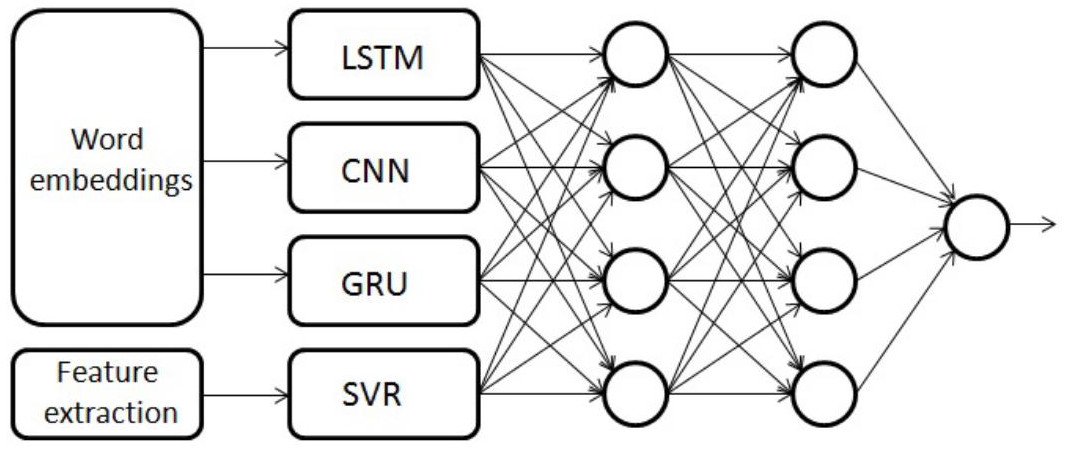
\includegraphics[width=0.8\textwidth]{MLPENSEMBLE}
    \caption{ ترکیب بر اساس MLP }
    \label{fig:MLP-ensemble}
\end{figure}

در این شبکه از نتایج شبکه‌های
LSTM
،
CNN
و 
GRU
استفاده شده‌است و با اضافه کردن تعدادی لایه‌ی
fully-connected
نتیجه‌ی نهایی ایجاد می‌شود.

\section{ روش‌های چندمنظوره }

\cite{kalchbrenner-etal-2014-convolutional} 3285 2014

\subsection{بررسی چند مقاله}


\chapter{جمع‌بندی و نتیجه‌گیری}
\pagebreak
\section{مقدمه}

\begin{latin}
    \bibliography{bibliography}
\end{latin}

\end{document}
